% FACTORIE User's Guide
% Copyright (c) 2009-. University of Massachusets, Department of Computer Science.
% Released under the Creative Commons 3.0 BY License.

%
% This manual is currently unfinished.  
% When it has more useful content, it will be directly linked from the
% FACTORIE web site.
%



\documentclass[]{manual}

% Use utf-8 encoding for foreign characters
\usepackage[utf8]{inputenc}
%\usepackage[T1]{fontenc}
%\usepackage[bitstream-charter]{mathdesign}

% Setup for fullpage use
\usepackage{fullpage}
\usepackage{amsmath}
\usepackage{epsfig}
\usepackage{color}
%\usepackage{pdfsync}

% Flexible citation syntax
\usepackage{natbib}

% Multipart figures
%\usepackage{subfigure}

% More symbols
\usepackage{amsmath}
\usepackage{amssymb}
\usepackage{latexsym}

% Line numbering
\usepackage{lineno}

% Package for including code in the document
\usepackage{listings}

% Surround parts of graphics with box
\usepackage{boxedminipage}

\usepackage{upquote}

% This is now the recommended way for checking for PDFLaTeX:
%\usepackage{ifpdf}

% Enable hyperlinks
\definecolor{Red}{rgb}{0.5,0,0}
\definecolor{Blue}{rgb}{0,0,0.5}
\usepackage[pdfpagemode=FullScreen,colorlinks=true,linkcolor=Red,citecolor=Blue,urlcolor=Red]{hyperref}

\newcommand{\cut}[1]{}


%\ifpdf
%\usepackage[pdftex]{graphicx}
%\else
%\usepackage{graphicx}
%\fi


\title{FACTORIE User's Guide:\\
Probabilistic Programming via Imperatively Defined Factor Graphs}
\author{Andrew McCallum \\ Karl Schultz \\ Sameer Singh \\ Sebastian Riedel \\ Michael Wick}
\graphicspath{{figs/}}
\pdfoutput=1
%\release{0.8}
%\date


%%%%%%%%%%%%%%% Commands from rst2latex %%%%%%%%%%%%%%%%%%%%%%%%
\newcommand{\rubric}[1]{\subsection{#1}}
\newcommand{\titlereference}[1]{\textsl{#1}}
\newlength{\locallinewidth}
\setlength{\locallinewidth}{7in}
\newlength{\admonitionwidth}
\setlength{\admonitionwidth}{0.9\textwidth}
%%%%%%%%%%%%%%%%%%%%%%%%%%%%%%%%%%%%%%%%%%%%%%%%%%%%%%%%%%%%%%%%%
\setcounter{secnumdepth}{1}


\begin{document}

\maketitle

\tableofcontents
%\linenumbers

% Examples to consider including:
% <h2>Coin Flips</h2>
% <h2>Rain, Sprinkler and Wet Grass</h2>
% <h2>Document Clustering with a Mixture of Multinomials</h2>
% <h2>Latent Dirichlet Allocation</h2>
% <h2>Smoking, Cancer and Friendships</h2>
% <h2>Companies, Employers and Respect</h2>
% <h2>Named Entity Recognition with Linear-chain CRFs</h2>
% <h2>Entity Resolution</h2>
% <h2>Dependency Parsing</h2>

\chapter{Introduction}
\label{chap:intro}

An overview of FACTORIE and its features.

\chapter{Installation}
\label{chap:install}

Where to find FACTORIE.  How to install it.  Where to find updates.
Where to find other users, discussion groups.  How to report errors
and suggestions.


\chapter{Tutorial}
\label{chap:tutorial}

A tutorial, based on multiple examples.  Show examples of
entity-relationship style of template definition, logic syntactic
sugar, and underlying imperative style.  Show examples of both
undirected and directed models.


\section{Entity Resolution with first order features - Toy Dataset}
(CorefMentions.scala)

\lstset{% general command to set parameter(s) 
basicstyle=\small, % print whole listing small 
keywordstyle=\color{black}\bfseries\underbar, 
% underlined bold black keywords 
identifierstyle=, % nothing happens 
commentstyle=\color{white}, % white comments 
stringstyle=\ttfamily, % typewriter type for strings 
showstringspaces=false} % no special string spaces 



In this section of the tutorial we will apply Factorie to the problem
of entity resolution (or coreference). \cut{Entity resolution is a problem
studied in many scientific communities, including natural language
processing, information extraction, data mining, and information
integration, as well as industry.} Informally, entity resolution is the
problem of clustering {\em mentions} into underlying {\em
  entities} (see Figure~\ref{fig:tutorial-coref-toy-data}).


\cut{Throughout this section we will highlight the power of several of
Factorie's types of imperativisms, including variable coordination,
online constraint preservation,sufficient statistics mapping, and
unrolling.}


\begin{figure}[h]
\begin{center}
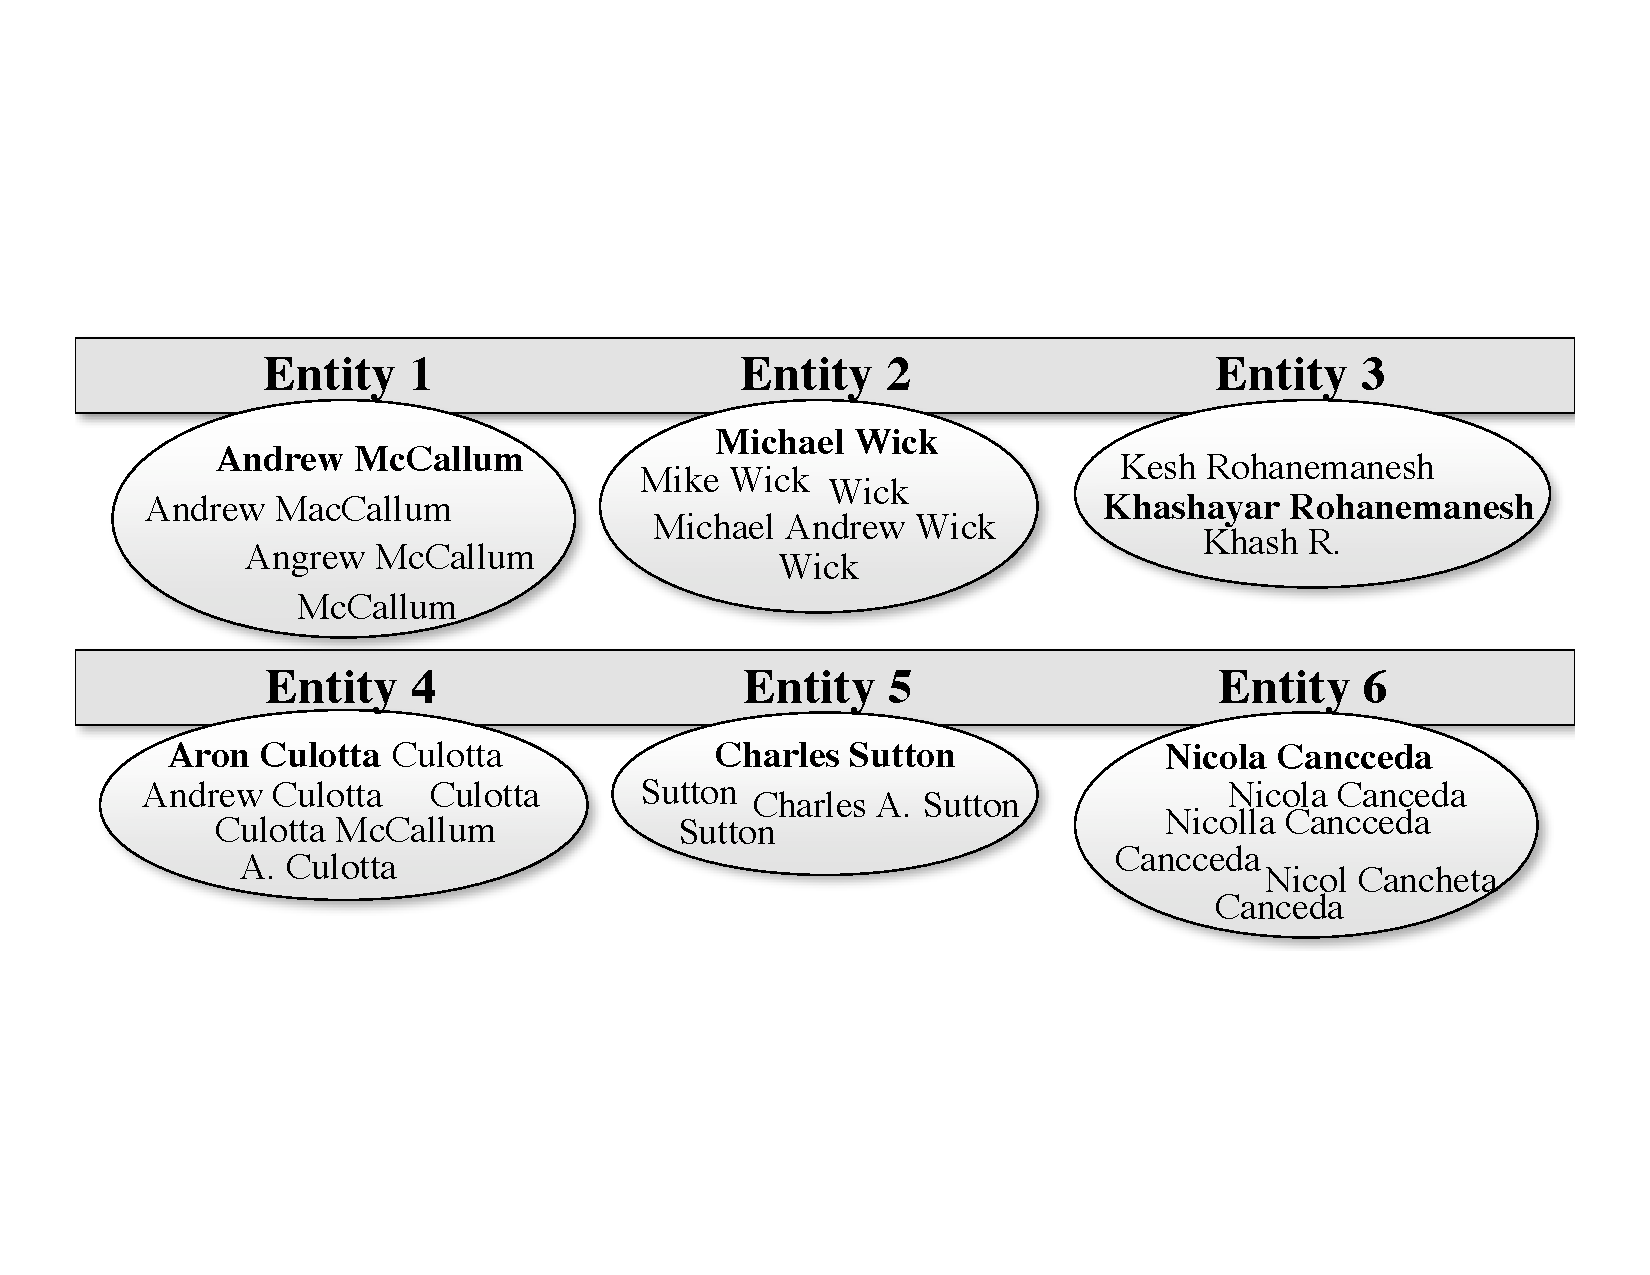
\includegraphics[width=0.88 \textwidth]{figs/coref-toy-data}
\caption{Ground truth toy coreference data. Bolded mentions are canonical (entity) names for cluster.}
\label{fig:tutorial-coref-toy-data}
\end{center}
\end{figure}


\subsection{Step 1: Define data structures and variables}
Before defining the structure of our model, we must
first create the basic data structures and random variables that
naturally support coreference data. We begin by defining a mention
variable:

\lstinline!class Mention(val name:String, val trueEntity:Int, val initialEntity) extends RefVariable(initialEntity)!

\noindent the Mention has three members: a name containing the text
(e.g., ``Aron Culotta''), a {\em trueEntity} used for supervised
training and evaluation, and an {\em initialEntity} used for defining
the initial configuration. The Mention additionally extends {\em
  RefVariable}, a factorie trait for variables whose possible values
points to scala objects; in our case, a setting to the mention
variable is a pointer to some entity in our hypothesis (by convention
all mentions with a pointer to the same entity will be considered
coreferent); we are now ready to define the {\em Entity} variable:

\begin{lstlisting}
class Entity(val canonical:String) extends SetVariable[Mention] {
  def mentions = members //for readability
  override def toString = "Entity("+canonical+":"+mentions.toSeq.size+")"
}
\end{lstlisting}

\subsection{Step 2: Define the factors}

Traditional machine learning approaches to coreference have modeled
dependencies between mention pairs. The approach of
\citep{soon01machine} treat each mention pair as an independent
classification decision. We begin our model description by expressing such a
factor.




\subsection{Step 3: Enforce structural constraints}
Since each mentions can only reference a single entity, an equivalance relation is enforced. Unfortunately, 


-up to this point we have defined most of the factor graph
-still need to enforce deterministic constraints
-introducing... constraint preservation.. staying in the feasible region



28 mentions, 6 entities. Number of configurations: Bell(28) = 

While this toy dataset only contains 28 mentions and 6 entities, the
network described in this chapter is actually impossible to fully
grounded in memory. The reason is that the first-order-logic feature over clusters would have to be evaluated for all possible entities, for which there are $2^{28}$

\subsection{Step 4: Instantiate data structure}

\subsection{Step 5: }

\chapter{Variables and Domains}
\label{chap:variables}

Objects representing random variables.

\section{The Basic Variable Classes}
\section{Defining Your own Variable Classes}
\section{Defining a Variable's Domain}
\section{Variables of Generative Models}
\section{Generative Distributions}


\chapter{Defining Models with Factor Templates}
\label{chap:models}


\chapter{Inference}
\label{chap:inference}

Sampling, MCMC, variational, maximization.


\chapter{Learning}
\label{chap:learning}

Objective functions as models. SampleRank, contrastive divergence (persistent variant?), structured perceptron, reinforcement learning(?).


\chapter{Diagnostics}
\label{chap:diagnostics}

\chapter{Database Back-end}
\label{chap:database}

\chapter{Conclusion}
\label{chap:conclusion}


% \appendix
% \chapter{Appendix: Foo}

\bibliographystyle{plainnat}
\bibliography{factorie-users-guide}

\end{document}
